\subsection{Aufgabe 1}
\begin{frame}{Aufgabe 1}
\begin{figure}[h!]
		\centering
		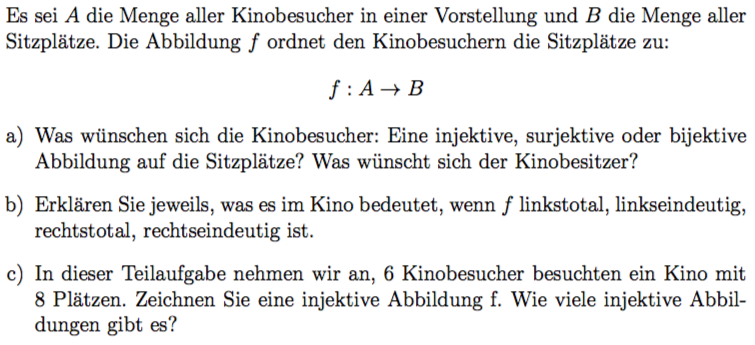
\includegraphics[width=\textwidth]{../topics/weihnachtstut-aufgaben/1.png} 
	\end{figure}     
\end{frame}

\begin{frame}{Aufgabe 1}
\begin{figure}[h!]
		\centering
		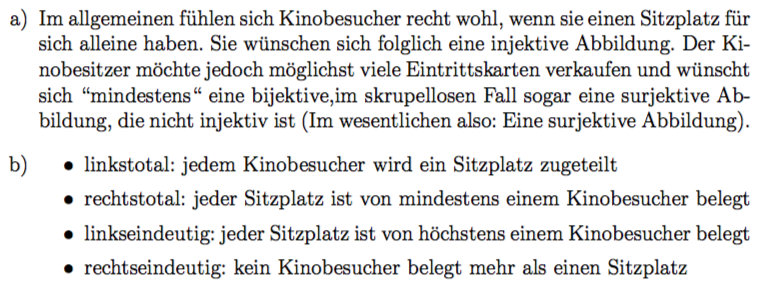
\includegraphics[width=\textwidth]{../topics/weihnachtstut-aufgaben/2.png} 
	\end{figure}  
	\begin{figure}[h!]
		\centering
		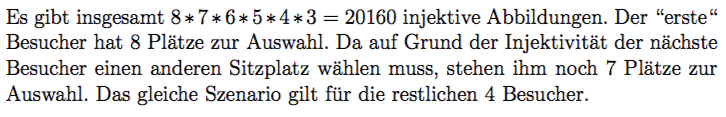
\includegraphics[width=\textwidth]{../topics/weihnachtstut-aufgaben/3.png} 
	\end{figure}   
\end{frame}

\subsection{Aufgabe 2}
\begin{frame}{Aufgabe 2}
\begin{figure}[h!]
		\centering
		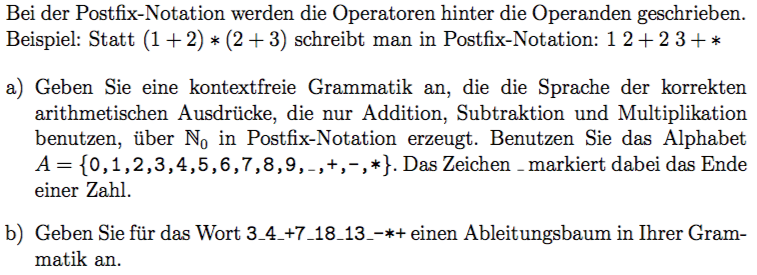
\includegraphics[width=\textwidth]{../topics/weihnachtstut-aufgaben/4.png} 
	\end{figure}     
Vermeide führende Nullen!
\end{frame}

\begin{frame}{Aufgabe 2}
\begin{figure}[h!]
		\centering
		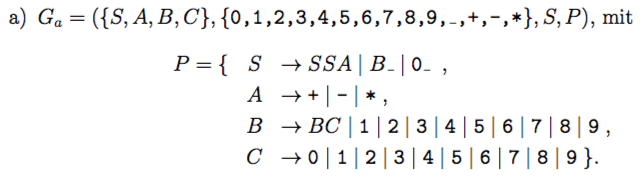
\includegraphics[width=\textwidth]{../topics/weihnachtstut-aufgaben/5.png} 
	\end{figure}    
\end{frame}

\subsection{Aufgabe 3}
\begin{frame}{Aufgabe 3}
\begin{figure}[h!]
		\centering
		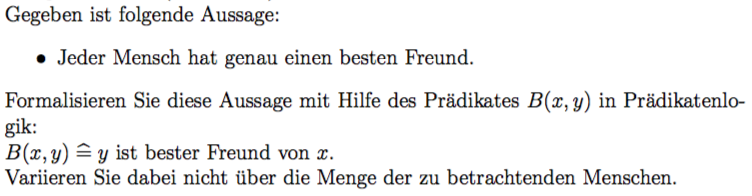
\includegraphics[width=\textwidth]{../topics/weihnachtstut-aufgaben/6.png} 
	\end{figure}     
\end{frame}

\begin{frame}{Aufgabe 3}
\begin{figure}[h!]
		%\centering
		%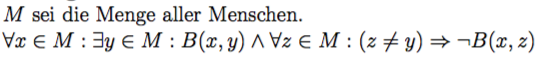
\includegraphics[width=\textwidth]{../topics/weihnachtstut-aufgaben/7.png} 
	\end{figure}    
		$M(x)$: \enquote{x ist ein Mensch} \\[1em]
		\[ \forall x (M(x) \rightarrow \exists y (M(y) \wedge B(x,y) \wedge \forall z (\neg (z \doteq y) \rightarrow \neg B(x,z))) \]
\end{frame}

\subsection{Aufgabe 4}
\begin{frame}{Aufgabe 4}
\begin{figure}[h!]
		\centering
		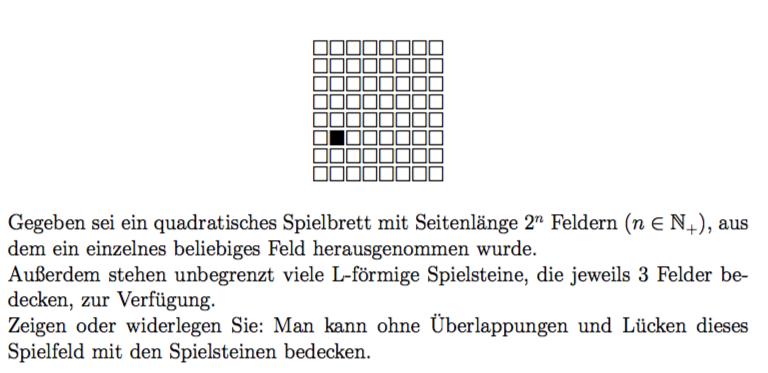
\includegraphics[width=\textwidth]{../topics/weihnachtstut-aufgaben/8.png} 
	\end{figure}     
\end{frame}

\begin{frame}{Aufgabe 4}
\begin{figure}[h!]
		\centering
		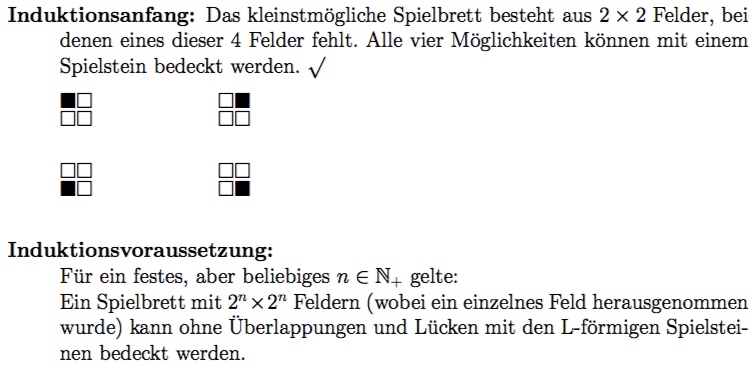
\includegraphics[width=\textwidth]{../topics/weihnachtstut-aufgaben/9.png} 
	\end{figure}    
\end{frame}

\begin{frame}{Aufgabe 4}
\begin{figure}[h!]
		\centering
		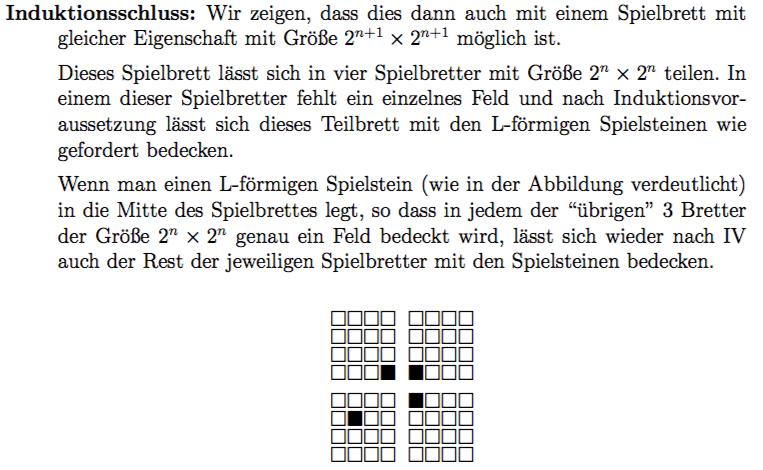
\includegraphics[width=\textwidth]{../topics/weihnachtstut-aufgaben/10.png} 
	\end{figure}    
\end{frame}

\subsection{Aufgabe 5}
\begin{frame}{Aufgabe 5}
\begin{figure}[h!]
		\centering
		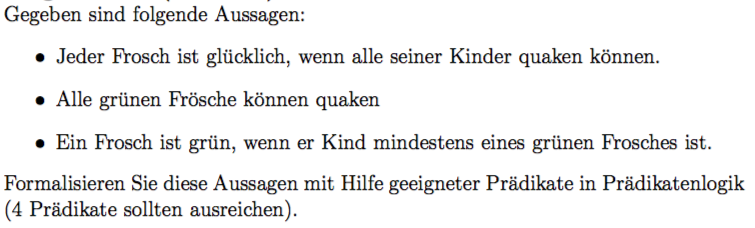
\includegraphics[width=\textwidth]{../topics/weihnachtstut-aufgaben/11.png} 
	\end{figure}     

	Wir wollen bei dieser Aufgabe die korrekte Notation etwas dehnen und erlauben die (in der intuitiven Bedeutung äquivalenten) Schreibweisen\footnote{vgl. Foliensatz Prädikatenlogik, Folie 44}:
	\begin{itemize}
		\item $\forall x \in F: \dots$ \quad statt \quad $\forall x (p(x) \rightarrow \dots) \quad \text{mit } I(p) = F \subseteq D.$
		\item $\exists x \in F: \dots$ \quad statt \quad $\exists x (p(x) \wedge \dots) \quad \text{mit } I(p) = F \subseteq D.$
	\end{itemize}

\end{frame}

\begin{frame}{Aufgabe 5}
\begin{figure}[h!]
		\centering
		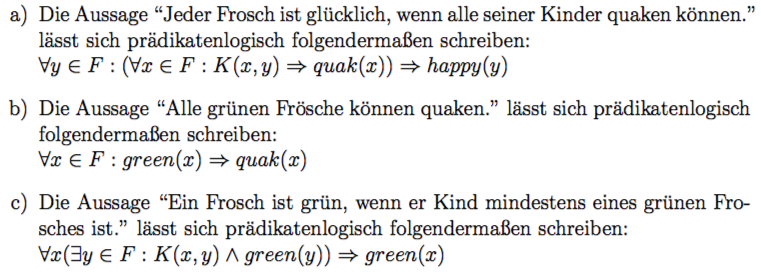
\includegraphics[width=\textwidth]{../topics/weihnachtstut-aufgaben/12.png} 
\end{figure} 

\end{frame}   
   	
\begin{frame}{Aufgabe 5}
	
		Die Notation oben ist natürlich nicht in unserem Sinne, aber mit der korrekten Notation wird es unübersichtlich: \\[1em]

		\begin{enumerate}
			\item \enquote{Jeder Frosch ist glücklich, wenn alle seine Kinder quaken können.} \\[.3em]
				\[ \forall y (F(y) \rightarrow ((\forall x ((F(x) \rightarrow K(x,y)) \rightarrow quak(x) )) \rightarrow happy(y))) \]
		\end{enumerate}

\end{frame}

\subsection{Aufgabe 6}
\begin{frame}{Aufgabe 6}
\begin{figure}[h!]
		\centering
		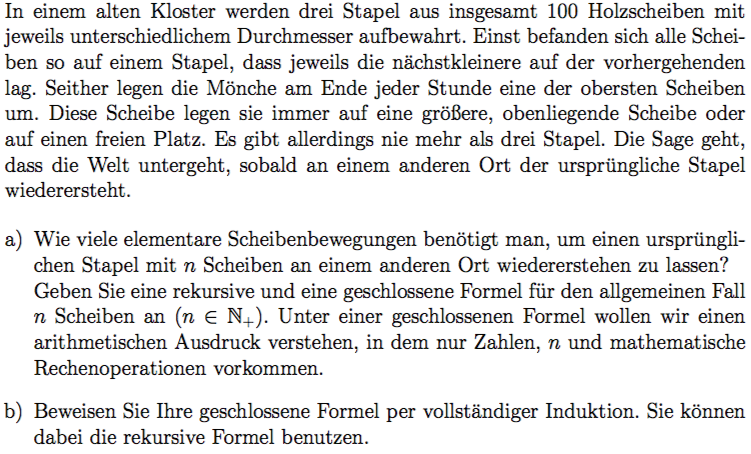
\includegraphics[width=\textwidth]{../topics/weihnachtstut-aufgaben/13.png} 
	\end{figure}     
\end{frame}

\begin{frame}{Aufgabe 6}
\begin{figure}[h!]
		\centering
		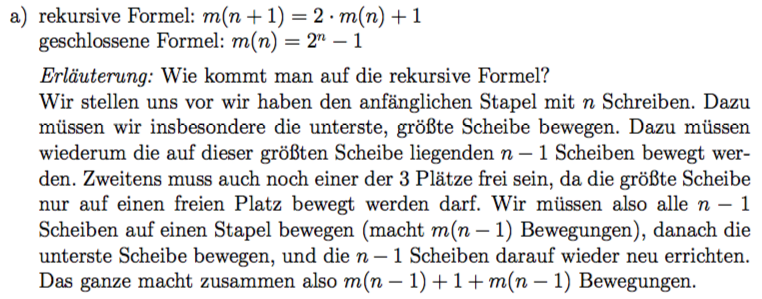
\includegraphics[width=\textwidth]{../topics/weihnachtstut-aufgaben/14.png} 
	\end{figure}     
\end{frame}

\begin{frame}{Aufgabe 6}
\begin{figure}[h!]
		\centering
		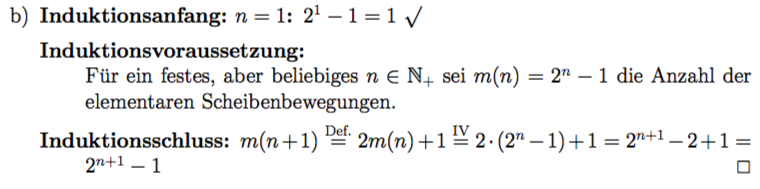
\includegraphics[width=\textwidth]{../topics/weihnachtstut-aufgaben/15.png} 
	\end{figure}     
\end{frame}

\begin{frame}{Aufgabe 6}
\begin{figure}[h!]
		\centering
		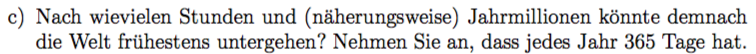
\includegraphics[width=\textwidth]{../topics/weihnachtstut-aufgaben/16.png} 
	\end{figure}     
\end{frame}

\begin{frame}{Aufgabe 6}
\begin{figure}[h!]
		\centering
		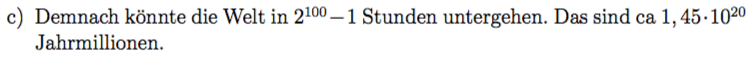
\includegraphics[width=\textwidth]{../topics/weihnachtstut-aufgaben/17.png} 
	\end{figure}     
\end{frame}

\subsection{Aufgabe 7}
\begin{frame}{Aufgabe 7}
\begin{figure}[h!]
		\centering
		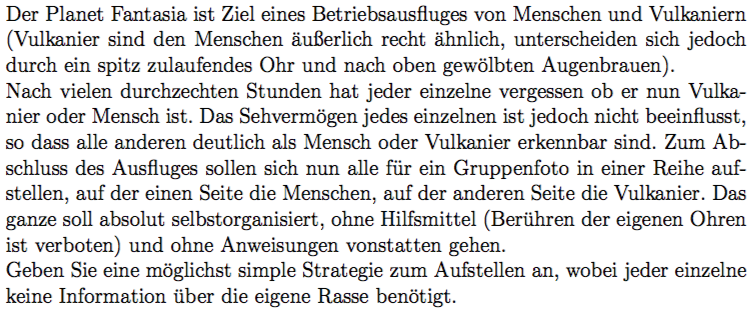
\includegraphics[width=\textwidth]{../topics/weihnachtstut-aufgaben/18.png} 
	\end{figure}     
\end{frame}

\begin{frame}{Aufgabe 7}
\begin{figure}[h!]
		\centering
		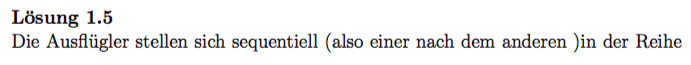
\includegraphics[width=\textwidth]{../topics/weihnachtstut-aufgaben/19.png} 
	\end{figure}  
	\begin{figure}[h!]
		\centering
		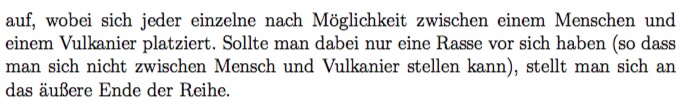
\includegraphics[width=\textwidth]{../topics/weihnachtstut-aufgaben/20.png} 
	\end{figure}   
\end{frame}